\chapter{A Chapter}

\lipsum[1] \ref{fig:frog}.

\begin{figure}
    \centering
    \caption{\label{fig:frog}This frog was uploaded via the file-tree menu.}
    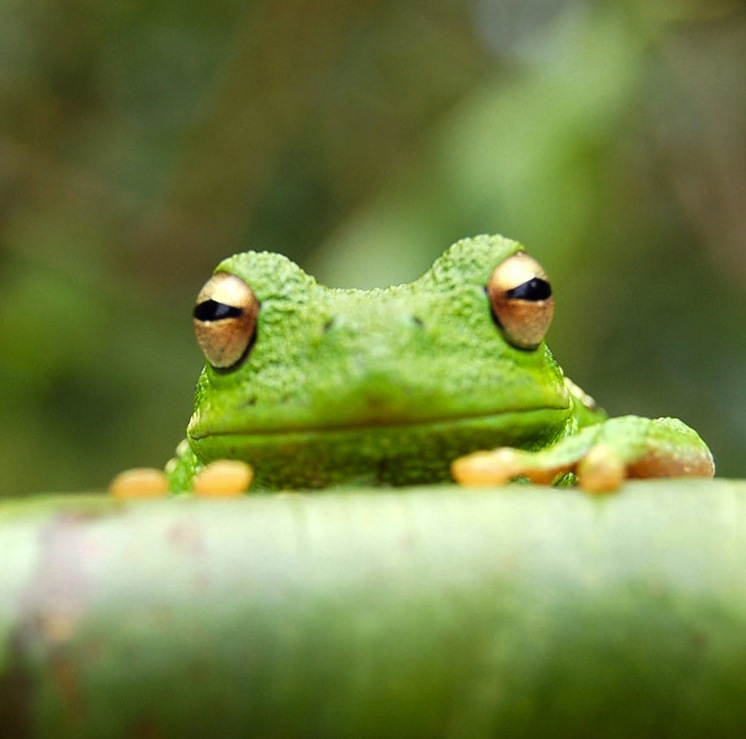
\includegraphics[width=0.3\textwidth]{frog.jpg}
\end{figure}

\section{A Section}

\lipsum[2]\footnote{footnotes working fine}\footnote{footnotes are working fine?}\footnote{lets hope footnotes working fine}

\section{B Section}

\subsection{A Subsection}
\lipsum[3]
\subsubsection{A Subsubsection}
\lipsum[4]
\subsection{B subsection}
\lipsum[5]\footnote{footnotes working fine}\footnote{footnotes are working fine?}\footnote{lets hope footnotes working fine}

\section{C Section}
\lipsum[6-8] \ref{tab:widgets} \cite{One, Two, Three}.

\begin{table}
    \centering
    \caption{\label{tab:widgets}An example table.}
    \begin{tabular}{l|r}
        Item & Quantity \\\hline
        Widgets & 42 \\
        Gadgets & 13
    \end{tabular}
\end{table}